%% Borrador para HardwareX (Elsevier). Estructura según la plantilla de la
%% revista: tabla de especificaciones, contexto, descripción, archivos de
%% diseño, lista de materiales, armado, operación y validación.
%%
%% Todo lo que está en rojo (\TODO{...}) falta: datos que solo se obtienen
%% midiendo en el microscopio, decisiones de los autores o archivos que
%% todavía no existen. No hay ningún número inventado: los valores que
%% aparecen salen del código o de mediciones documentadas en el repositorio
%% (se indica de dónde). Ver LEEME.md.
\documentclass[preprint,12pt]{elsarticle}

\usepackage[T1]{fontenc}
\usepackage[utf8]{inputenc}
\usepackage{lmodern}
\usepackage{amsmath}
\usepackage{graphicx}
\usepackage{booktabs}
\usepackage{tabularx}
\usepackage{longtable}
\usepackage{array}
\usepackage{xcolor}
\usepackage{textcomp}
\usepackage{url}
\expandafter\def\expandafter\UrlBreaks\expandafter{\UrlBreaks\do\_\do\:\do\[}
\Urlmuskip=0mu plus 2mu
\usepackage[hidelinks]{hyperref}

\DeclareRobustCommand{\TODO}[1]{\textcolor{red}{\textbf{[TODO\ifx\relax#1\relax\else: #1\fi]}}}
\newcommand{\um}{\,\textmu m}
\newcolumntype{L}{>{\raggedright\arraybackslash}X}

\graphicspath{{../capturas/}}

\journal{HardwareX}

\begin{document}

\begin{frontmatter}

\title{MicroscopeOS: an open, incubator-integrated, dual-camera LED-array
microscope for label-free long-term live-cell imaging with phase-based
autofocus}

%% TODO: nombres reales, laboratorio, ciudad y correo.
\author[uanl]{Author One}
\author[uanl]{Author Two}
\author[uanl]{Corresponding Author\corref{cor1}}
\cortext[cor1]{Corresponding author: name@uanl.edu.mx}
\address[uanl]{Laboratory, Faculty, Universidad Autónoma de Nuevo León,
  City, Nuevo León, Mexico}

\begin{abstract}
Unstained living cells are phase objects: they barely absorb light and are
nearly invisible under brightfield illumination, precisely at focus.
Commercial live-cell imaging systems solve this inside the incubator, but
their cost keeps them out of reach of many laboratories. We present
MicroscopeOS, an open-source microscope built around a Raspberry Pi~5 that
images two independent samples inside a temperature- and CO$_2$-controlled
chamber for time-lapse experiments of up to 48~h. Each optical channel has
its own 8~MP camera, a programmable $8\times8$ RGB LED array driven by an
ESP32-S3 microcontroller, and a motorised focus axis. The LED arrays provide
brightfield, darkfield, Rheinberg and differential phase contrast (DPC)
illumination without moving parts. The same half-aperture illumination used
for DPC drives a two-stage autofocus: the signed lateral shift between the
two half-aperture images indicates both the direction and the magnitude of
defocus, so the system refocuses without blind sweeps. DPC images are
computed on the Raspberry Pi at the end of every cycle, reducing storage
from $\sim$65~MB to $\sim$25~MB per camera and cycle. The instrument is
operated from a web interface designed for first-time users, accessible on
the local network or remotely through an authenticated tunnel, and streams
every image to a GPU workstation for live segmentation. All software,
firmware and a hardware-free test suite with physics-based emulators are
openly available. \TODO{One sentence with the main validation results
(resolution, autofocus repeatability, 48~h stability, cell viability).}
\end{abstract}

\begin{keyword}
Open hardware \sep Live-cell imaging \sep Differential phase contrast \sep
LED array microscopy \sep Autofocus \sep Raspberry Pi \sep Time-lapse
\sep Incubator microscope
\end{keyword}

\end{frontmatter}

%% ---------------------------------------------------------------------------
\section*{Specifications table}

\noindent
\begin{tabularx}{\textwidth}{>{\raggedright\arraybackslash}p{0.3\textwidth}L}
\toprule
Hardware name & MicroscopeOS \\
Subject area & Biological sciences (e.g., microbiology and biochemistry);
  Educational tools and open source alternatives to existing infrastructure \\
Hardware type & Imaging tools \\
Closest commercial analog & Incubator live-cell imaging systems such as
  Sartorius Incucyte or CytoSMART Lux \TODO{confirm and cite the closest
  model and its price} \\
Open source license & \TODO{Choose and add LICENSE files to the repository.
  Suggested: GPL-3.0 (software and firmware) and CERN-OHL-S-2.0 (hardware
  design files)} \\
Cost of hardware & \TODO{Total from the bill of materials, in USD} \\
Source file repository & \TODO{Zenodo/OSF/Mendeley Data DOI (HardwareX does
  not accept GitHub alone)}; development repository:
  \url{https://github.com/AFMMenchacalab/microscopeos-pi5} \\
\bottomrule
\end{tabularx}

%% ---------------------------------------------------------------------------
\section{Hardware in context}

Directional and random cell migration underlies development, wound healing
and cancer invasion \cite{Ref003}, and measuring it requires imaging living
cells for many hours under physiological conditions, then segmenting and
tracking them \cite{WuWirtz2026Methods}. Two difficulties make this
expensive. First, the cells must stay at 37\,\textdegree C and controlled
CO$_2$ for the whole experiment, which means placing the microscope inside
an incubator or building an incubator around it. Second, unstained cells
are phase objects: they delay the wavefront rather than absorb it, so in
brightfield their contrast is proportional to defocus and vanishes at
focus. Fluorescent labels solve the contrast problem but add phototoxicity
over long acquisitions \cite{Icha2017,Laissue2017}. Classical phase
contrast \cite{Zernike1942} and asymmetric illumination
\cite{Kachar1985,Mehta2009} recover contrast optically, and programmable
LED arrays made these modalities, including quantitative differential phase
contrast (DPC), available in software without dedicated optics
\cite{Zheng2011LED,Liu2014LED,Tian2014DPC3D,Tian2015DPC,Lee2015Color,Chen2018DPCaberr}.

Commercial incubator microscopes integrate these pieces, but at a price
that limits access, a recurring argument for open instrumentation
\cite{Ref027,Ref024,Ref023,Ref026}. Open microscopes are now mature
platforms: OpenFlexure \cite{Collins2020OFM}, UC2 \cite{Ref040}, the
\texteuro100 lab \cite{Ref043}, PlanktoScope \cite{Ref036}, ESPressoscope
\cite{Ref032}, Trackoscope \cite{Ref029} and automated open fluorescence
microscopes \cite{Ref030}, and low-cost LED-array computational microscopy
has been demonstrated on Raspberry Pi hardware \cite{Ref042}. For long-term
live imaging, the Incubot places a 3D-printer-based microscope inside a
culture incubator \cite{Merces2021}; other works provide open
temperature or CO$_2$ control \cite{OCarroll2023,Talebipour2024,Rossi2022,
Chen2021PrintrLab}, adapt OpenFlexure to live cells \cite{Kearns2026OFMLive}
or build 3D-printed in-incubator time-lapse platforms \cite{Sato2026DIY}.
Reproducibility of such instruments depends on publishing complete design
files and validation \cite{Ref025}.

To our knowledge, no open instrument combines, in a single device: (i) two
independent optical channels, so that two conditions are imaged in the same
experiment; (ii) label-free computational contrast (DPC, darkfield and
Rheinberg) from a programmable LED array per channel; (iii) an autofocus
that reuses the DPC illumination to obtain the \emph{direction} of defocus,
building on illumination-based autofocus for slide scanning
\cite{Liao2016Autofocus} rather than on image-sharpness sweeps or trained
networks \cite{Pinkard2019,Luo2021Autofocus}; (iv) environmental control
logged with every frame; and (v) on-device processing, data offload and
authenticated remote operation for unattended experiments.
\TODO{Check this claim against the latest literature before submission.}

%% ---------------------------------------------------------------------------
\section{Hardware description}

MicroscopeOS (Fig.~\ref{fig:architecture}) is organised in five subsystems
that communicate with a Raspberry Pi~5, which runs all acquisition,
processing and the web server.

\begin{figure}[ht]
\centering
\fbox{\parbox[c][5cm][c]{0.9\textwidth}{\centering
\TODO{Architecture diagram: Raspberry Pi 5 at the centre; CSI to the two
IMX219 cameras; USB serial to the two ESP32-S3 LED arrays; shared UART bus
to the two TMC2209 drivers and NEMA 11 motors; USB serial to the Arduino
with DS18B20, SCD30, heater and CO$_2$ valve; network to the browser, the
GPU workstation, the NAS and the remote-access tunnel. The ASCII version is
in the repository README.}}}
\caption{System architecture.}
\label{fig:architecture}
\end{figure}

\paragraph{Imaging} Each channel uses a Raspberry Pi Camera Module~2
(Sony IMX219, $3280\times2464$ pixels, 1.12\um{} pixel pitch) on its own
CSI port of the Raspberry Pi~5, so both cameras capture truly in parallel
without a multiplexer. Images are saved as 16-bit TIFF files at the native
sensor resolution from the raw Bayer data. \TODO{Describe the objective
(currently configured as 20$\times$/NA~0.4 in \path{core/optica.py}), tube
lens or adapter, and the optical path; give the measured
\textmu m/pixel from a stage micrometer.}

\paragraph{Programmable illumination} Each channel has a Waveshare
ESP32-S3-Matrix board with an $8\times8$ WS2812B RGB LED array below the
sample. The microcontroller runs custom firmware
(\path{codigo/extras/matrices_esp32s3_matrix/}) that receives
line-based commands over USB serial (\path{PATTERN:brightness[:RRGGBB]})
and acknowledges each one. Patterns include full aperture (brightfield),
the four half apertures (left, right, top, bottom) for DPC, an outer ring
(darkfield) and a two-colour centre-plus-ring pattern (Rheinberg). Each
board is identified by a udev rule (\path{/dev/matriz_cam0},
\path{/dev/matriz_cam1}), independent of USB enumeration order.
\TODO{Distance from the array to the sample and the resulting
illumination NA.}

\paragraph{Focus actuation} Each channel has a NEMA~11 stepper motor
(28HB30-401A, 0.6~A/phase, 1.8\textdegree/step) on a T6$\times$1 lead-screw
linear stage, so one full step moves the stage 5\um{}; with the driver's
internal 1/256 microstepping the nominal resolution is $\sim$0.02\um.
Both motors are driven by TMC2209 drivers on a single shared UART bus in
multi-address mode, which lets the software change microstep resolution and
current on the fly and read the driver status. Backlash is avoided by
always approaching the final position from the same direction. There are no
limit switches; the software limits the total focus drift allowed during a
time-lapse to 250\um{} (\texttt{DERIVA\_MAXIMA\_UM}).

\paragraph{Environmental control} A separate Arduino (Uno/Nano) runs a PID
loop for temperature (DS18B20 sensor, PWM heater; setpoint 37\,\textdegree C,
output slew-rate limited to avoid overshoot) and a time-proportional PID for
CO$_2$ (Sensirion SCD30 sensor, solenoid valve; setpoint 4\%), and reports
telemetry as JSON over serial. Keeping the control loop on its own
microcontroller makes it independent of the Raspberry Pi's timing while it
writes 16~MB TIFF files. \TODO{Describe the chamber: volume, material,
insulation, heater power, CO$_2$ source and humidification.}

\paragraph{Computation and software} The Raspberry Pi~5 runs MicroscopeOS,
a Python application (FastAPI server, \texttt{picamera2}) started at boot
by systemd. The main software features are:
\begin{itemize}
\item \textbf{Time-lapse} with sequential or simultaneous capture of both
  cameras, per-cycle environmental telemetry, optional refocusing every
  $N$ cycles, and automatic resumption after a power cut (the Pi waits for
  network time synchronisation, since it has no real-time clock battery,
  and for the storage device to mount).
\item \textbf{DPC computed on the device} after every cycle
  (\path{core/dpc.py}): each half-aperture image is first normalised by
  its own low-pass background, because the two halves of the array differ
  in brightness by up to a factor of two in our assembly; then
  $\mathrm{DPC} = (I_L - I_R)/(I_L + I_R)$ and the analogous top--bottom
  image are stored as losslessly compressed 16-bit TIFFs together with a
  half-resolution brightfield sum. The four raw images are deleted only
  after the output has been verified on disk. Optionally, quantitative
  phase is retrieved by Tikhonov deconvolution with weak-object transfer
  functions \cite{Tian2015DPC}.
\item \textbf{Metadata in every image}: objective, pixel size,
  illumination, exposure, focus position, temperature and experiment, in
  ImageJ-compatible tags so that Fiji \cite{Ref079} opens each image with
  its physical scale, plus a JSON tag with the full record.
\item \textbf{Cell counting} on the live view and on captures, using a
  classical, non-learned detector of local energy at the cell scale, with a
  quality filter that distinguishes an empty field (or a switched-off lamp)
  from a confluent culture; in a time-lapse it produces a population curve
  and doubling time.
\item \textbf{Data offload}: each image is sent over the local network to
  a GPU workstation, discovered automatically by UDP broadcast and paired
  with a 6-digit code, where it is segmented on arrival with Cellpose-SAM
  \cite{Ref068,Pachitariu2025CellposeSAM}; transfers are verified by
  SHA-256 and queued, so a network outage neither stops nor loses the
  time-lapse. Images can also be backed up to a NAS over SMB or saved to a
  USB drive.
\item \textbf{Web interface} (Fig.~\ref{fig:ui}) organised in four numbered
  steps (turn on the light, look at the sample, focus, take a photo or a
  time-lapse), with simultaneous live view of both cameras, keyboard focus
  control, an image gallery and watermarked exports with a scale bar.
\item \textbf{Remote access}: the Raspberry Pi opens an outbound,
  encrypted tunnel (Cloudflare Tunnel), so no inbound port is opened on the
  institutional network; access is restricted to an allow-list of
  laboratory members who log in with a one-time code sent by e-mail
  (Cloudflare Access).
\end{itemize}

\begin{figure}[ht]
\centering
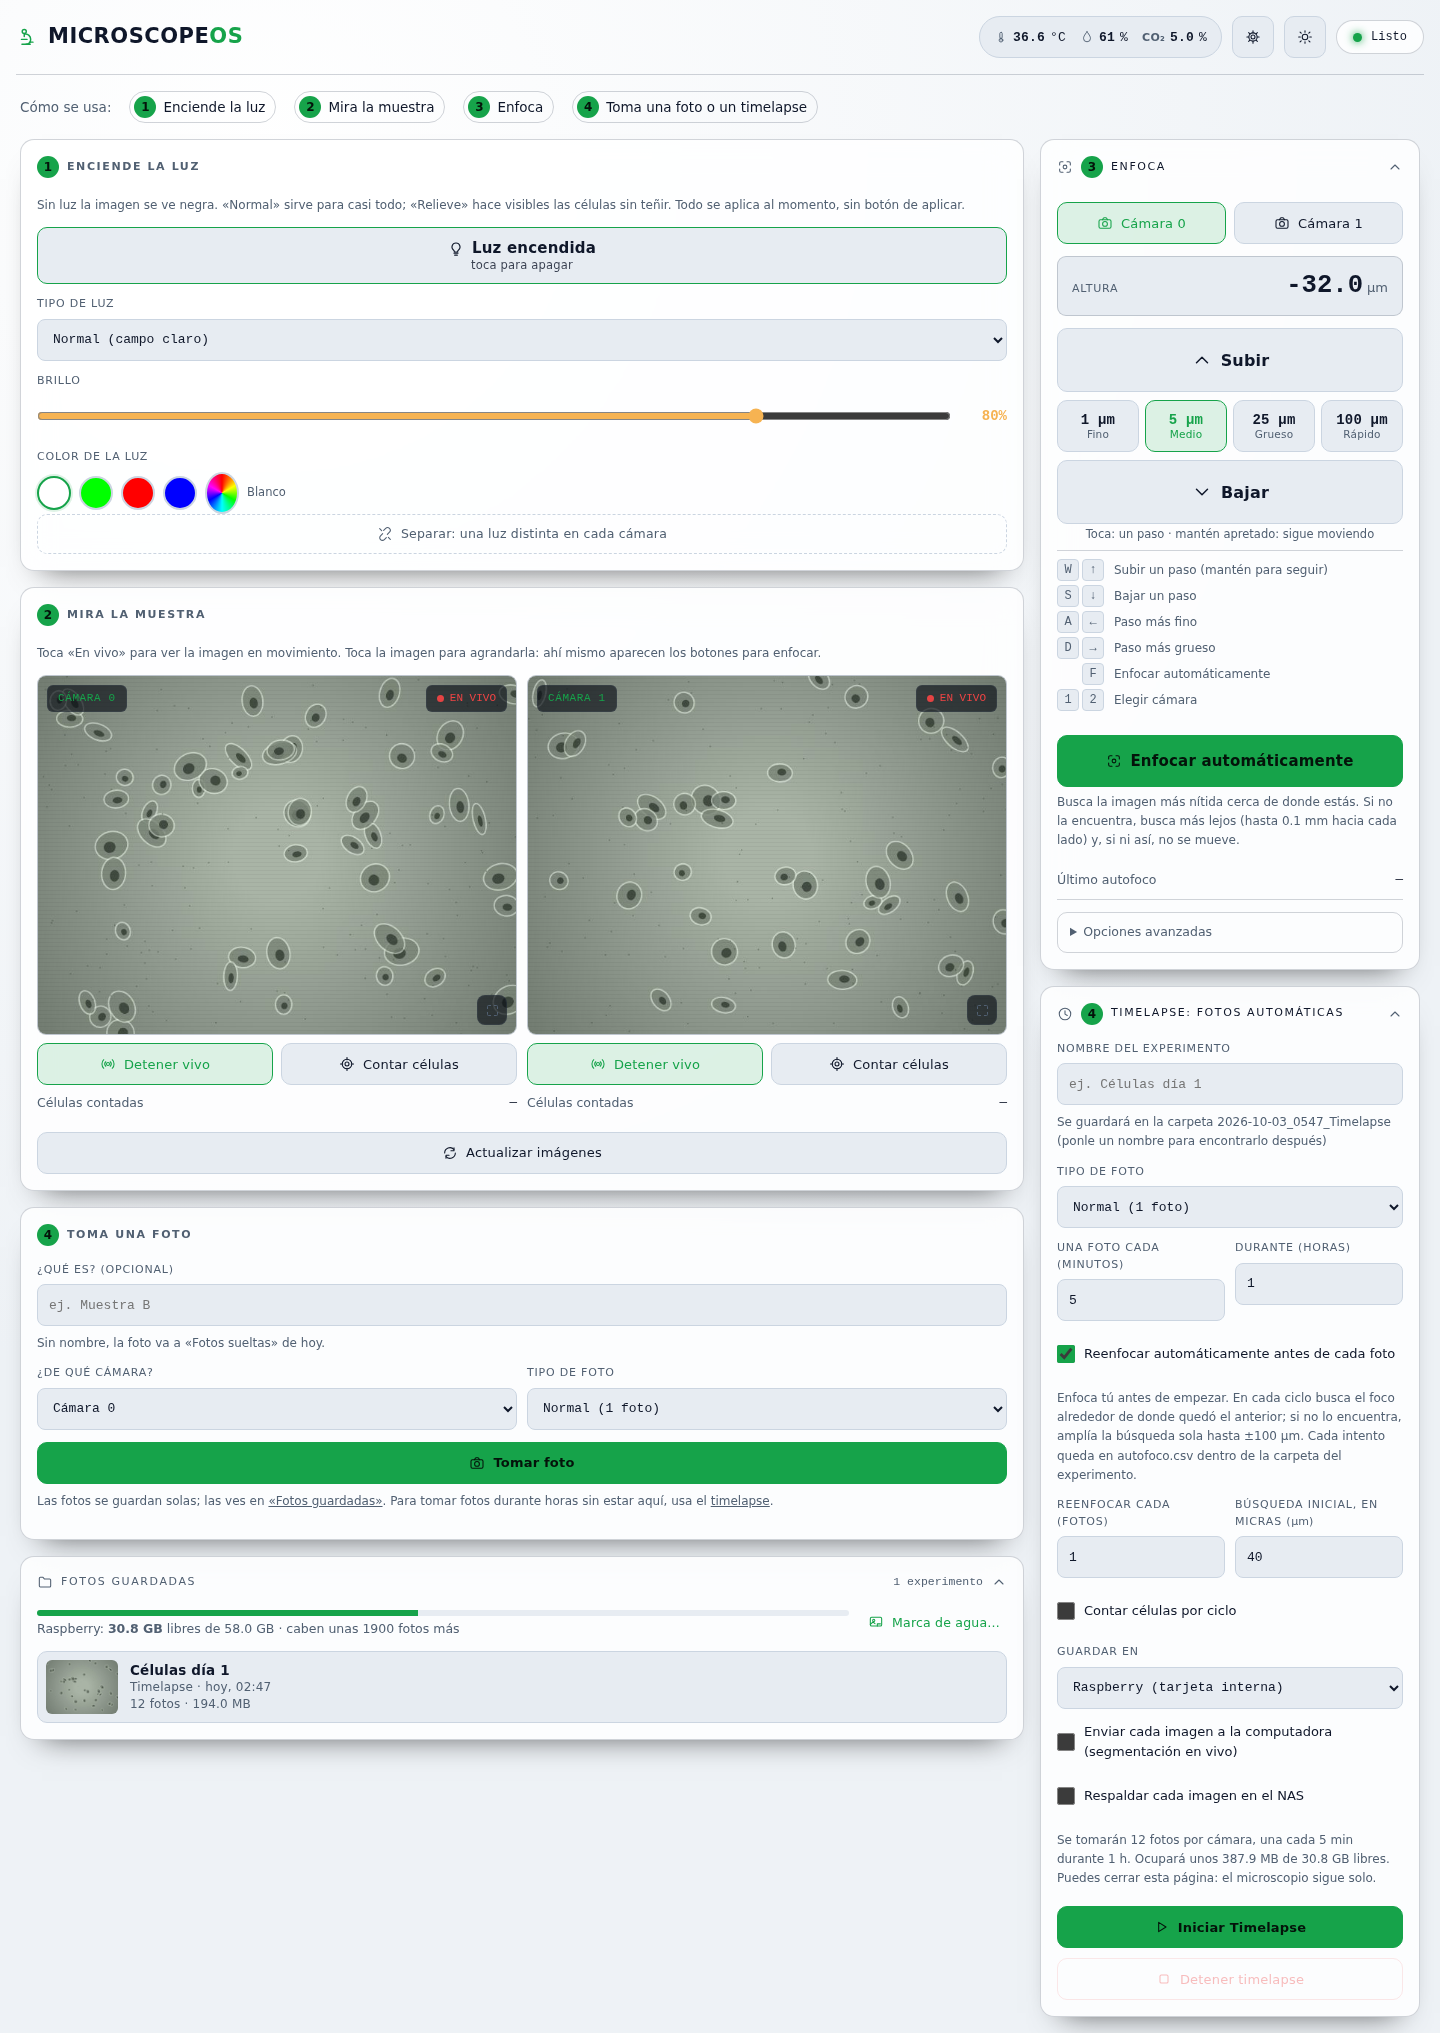
\includegraphics[width=0.9\textwidth,trim=0 1133 0 0,clip]{web_pagina.png}
\caption{Web interface. Screenshot taken with the simulated microscope used
to generate the user manual; the page is the same one served by the
instrument. \TODO{Replace or complement with a screenshot from the real
instrument showing real cells.}}
\label{fig:ui}
\end{figure}

\paragraph{Autofocus} Under half-aperture illumination, a defocused plane
is projected sideways, and in opposite directions for opposite halves of
the array. The lateral shift between the left and right images therefore
has a sign that indicates the direction of defocus, and within a linear
range its magnitude is proportional to the distance from focus. MicroscopeOS
estimates the shift by phase correlation with sub-pixel precision and
refocuses in two stages. (1) A coarse, directed jump: after a one-time
calibration per objective (a scan of $\pm$12\um{} that fits the
shift-versus-position line), a single measurement gives the distance to the
zero crossing, and the stage moves there directly. (2) Fine adjustment:
because a single reading is noisy close to focus, the shift is measured at
7 nearby planes and the median of the 7 zero-crossing estimates is taken.
If the system is uncalibrated, if the correlation is weak (empty field), or
if a correction moves away from focus, the stage returns to the start and a
coarse-to-fine sweep searches for the same criterion (the zero crossing of
the shift), so both methods converge to the same plane. The search starts at
$\pm$20\um{} and widens up to $\pm$100\um{} if needed. We deliberately avoid
image-sharpness metrics: the Tenengrad metric computed on DPC images is
almost flat near focus with unstained cells and shows a local
\emph{minimum} at focus with absorbing samples, which made sharpness-based
autofocus stop at a different plane in each run. The calibration span
($\pm$12\um) is chosen to stay inside the range where the shift is linear
($\sim\pm$15\um{} in our setup).

\paragraph{How this hardware helps researchers}
\begin{itemize}
\item It images two samples or conditions in parallel, each with its own
  focus and illumination, for up to 48~h under controlled temperature and
  CO$_2$.
\item It provides label-free contrast of unstained cells (DPC) without
  phase objectives, avoiding the phototoxicity of fluorescence.
\item It refocuses autonomously during long experiments, using the same
  illumination as the contrast mode.
\item Every image carries its physical scale and acquisition conditions,
  and the device reduces storage on the fly by computing DPC.
\item It is operated from any browser by users without prior training, on
  site or remotely, and streams images to a workstation for live analysis.
\item All software can be tested without hardware, using emulators of the
  camera (including DPC physics), LED arrays and motor drivers.
\end{itemize}

%% ---------------------------------------------------------------------------
\section{Design files summary}

\noindent
\begin{tabularx}{\textwidth}{>{\raggedright\arraybackslash}p{0.33\textwidth}
  >{\raggedright\arraybackslash}p{0.14\textwidth}
  >{\raggedright\arraybackslash}p{0.17\textwidth}L}
\toprule
Design file name & File type & Open source license & Location of the file \\
\midrule
MicroscopeOS (acquisition, processing, web server) & Python, HTML &
  \TODO{} & \path{codigo/MicroscopeOS/} \\
LED array firmware (\path{dpc_matrix.ino}) & Arduino (C++) &
  \TODO{} & \path{codigo/extras/matrices_esp32s3_matrix/} \\
Incubator PID firmware (\path{Control_Incubator_TempCO2.ino}) &
  Arduino (C++) & \TODO{} &
  \path{codigo/extras/incubadora_temperatura/} \\
Autofocus model training (optional) & Python & \TODO{} &
  \path{codigo/extras/ia/} \\
System configuration (boot, udev, systemd, tunnel example) & Text &
  \TODO{} & \path{configs/} \\
Hardware-free test suite and emulators & Python & \TODO{} &
  \path{tests/} \\
User manual & PDF, HTML & \TODO{} & \path{docs/instructivo/} \\
\TODO{Mechanical parts (camera mounts, sample holder, LED array holder,
  focus stage brackets)} & \TODO{STL + STEP} & \TODO{} &
  \TODO{not yet in the repository} \\
\TODO{Chamber design and wiring diagram} & \TODO{PDF/SVG} & \TODO{}
  & \TODO{not yet in the repository} \\
\bottomrule
\end{tabularx}

\medskip\noindent
\TODO{One sentence describing each design file, as required by the
journal.}

%% ---------------------------------------------------------------------------
\section{Bill of materials summary}

\noindent\TODO{Fill in unit costs and suppliers (marked ?) and part numbers. The components are those of the instrument as built.}
\medskip


\noindent
\begin{tabularx}{\textwidth}{>{\raggedright\arraybackslash}p{0.38\textwidth}
  >{\centering\arraybackslash}p{0.07\textwidth}
  >{\centering\arraybackslash}p{0.12\textwidth}
  >{\centering\arraybackslash}p{0.12\textwidth}L}
\toprule
Component & Qty & Unit cost (USD) & Total (USD) & Source \\
\midrule
Raspberry Pi 5 (8 GB) & 1 & ? & ? & ? \\
Raspberry Pi 5 power supply (27 W) & 1 & ? & ? & ? \\
microSD card / storage & 1 & ? & ? & ? \\
Raspberry Pi Camera Module 2 (IMX219) & 2 & ? & ? & ? \\
CSI cables for Raspberry Pi 5 & 2 & ? & ? & ? \\
Microscope objective \TODO{model} & 2 & ? & ? & ? \\
Waveshare ESP32-S3-Matrix ($8\times8$ WS2812B) & 2 & ? & ? &
  ? \\
NEMA 11 stepper motor 28HB30-401A & 2 & ? & ? & ? \\
Linear stage with T6$\times$1 lead screw (28T0601-50) & 2 & ? &
  ? & ? \\
TMC2209 stepper driver & 2 & ? & ? & ? \\
Motor power supply \TODO{voltage} & 1 & ? & ? & ? \\
Arduino Uno/Nano & 1 & ? & ? & ? \\
DS18B20 temperature sensor & 1 & ? & ? & ? \\
Sensirion SCD30 CO$_2$ sensor & 1 & ? & ? & ? \\
Heater \TODO{type, power} and MOSFET driver & 1 & ? & ? &
  ? \\
CO$_2$ solenoid valve and regulator & 1 & ? & ? & ? \\
Chamber, 3D-printed parts, fasteners & -- & ? & ? & ? \\
\midrule
\textbf{Total} & & & ? & \\
\bottomrule
\end{tabularx}

%% ---------------------------------------------------------------------------
\section{Build instructions}

\TODO{Step-by-step mechanical assembly with photographs: frame, focus
stages, camera and objective mounts, LED array holders, chamber, heater,
sensors and CO$_2$ line. HardwareX requires enough detail for someone else
to reproduce the instrument, including safety warnings.}

\paragraph{Electronics} \TODO{Wiring diagram.} The two TMC2209 drivers
share one UART line connected to GPIO14/15 of the Raspberry Pi, each
configured to a different address; the complete pin assignment is
documented in \path{core/motor_focus.py}. The LED arrays and the Arduino
connect by USB.

\paragraph{Software installation} On Raspberry Pi OS (64-bit), the
hardware-dependent packages (\texttt{picamera2}, OpenCV, NumPy, pyserial,
GPIO) are installed with \texttt{apt}, and the remaining dependencies in a
virtual environment that inherits the system packages. The boot
configuration enables both IMX219 cameras and the UART used by the
drivers, udev rules give the LED arrays stable names, and a systemd unit
starts the server at boot. The firmware for the LED arrays and the incubator
controller is flashed with the Arduino tool chain using the library
versions pinned in the repository. Remote access is configured with
\texttt{cloudflared}; an example configuration without credentials is
provided. Full commands are given in the repository README.

%% ---------------------------------------------------------------------------
\section{Operation instructions}

The instrument is operated from a web browser at the Raspberry Pi's
address. The interface guides the user through four steps: (1) turn on the
light and choose the illumination (normal brightfield, or ``relief''
(DPC) for unstained cells), brightness and colour; (2) start the live view
of each camera; (3) focus with buttons, the keyboard or the autofocus
button; (4) take a single image or configure a time-lapse (name,
illumination mode, interval, duration, refocusing, cell counting, storage
destination and optional transfer to the workstation and NAS). The
interface estimates the number of images and the disk space before
starting, and the time-lapse continues if the browser is closed. A
twelve-page printed manual for first-time users, including a
troubleshooting table and a quick-reference card, is provided in the
repository.

\paragraph{Safety}
\begin{itemize}
\item The focus axes have no limit switches; an excessive movement can
  drive the objective into the sample. Approach the sample manually before
  using autofocus. \TODO{Add mechanical end stops or describe the safe
  setup.}
\item The LED arrays are powered by USB; brightness is capped in software to
  keep current within the USB limit.
\item \TODO{Heater and CO$_2$ cylinder safety: over-temperature protection,
  pressure regulation and ventilation.}
\end{itemize}

%% ---------------------------------------------------------------------------
\section{Validation and characterization}

\paragraph{Validated so far} On the assembled instrument, both cameras
capture 16-bit TIFF images at native resolution in parallel; the four
illumination modes respond and were confirmed visually; both focus axes
move correctly through the shared UART bus; and remote access through the
tunnel was verified to redirect every unauthenticated request, including
motion commands, to the login page. The on-device DPC was measured on a
real capture of camera~0 ($3280\times2464$): each DPC image occupies
10.6~MB and the half-resolution brightfield sum 2.8~MB, $\sim$25~MB per
cycle and camera compared with $\sim$65~MB for the four raw images. The
pixel noise of the DPC image, measured in empty regions of the same sample,
was $\sim$0.008, which motivated storing DPC with a step of 1/4096 (the
quantisation adds about 1\% of that noise).

\paragraph{Software tests} The test suite runs without any hardware: it
replaces the camera, the LED arrays and the motor drivers with emulators
that speak the real protocols, including a camera model with DPC physics
(defocus, signed shift under half-aperture illumination, and phase objects
whose brightfield contrast vanishes at focus). In these simulations, a
sharpness sweep on raw brightfield images converges to a plane far from
focus, whereas the DPC-shift criterion converges to focus. On synthetic
fields of 40 phase cells in focus, the cell counter finds 0 cells under
brightfield and 40 under half-aperture or DPC illumination, which is why
live counting switches the array to half-aperture illumination. These
results are from simulation and must be confirmed on real samples.

\paragraph{Pending characterisation}
\TODO{Each item below needs an experiment and a figure. No values are
reported until they are measured.}
\begin{enumerate}
\item \textbf{Resolution and field of view}: USAF 1951 target under each
  illumination mode; stage micrometer for the \textmu m/pixel scale of
  each channel. \TODO{figure + table}
\item \textbf{DPC contrast}: the same field of unstained cells under
  brightfield, half aperture and DPC; optionally a phase reference
  (microspheres of known size and refractive index). \TODO{figure}
\item \textbf{Autofocus}: accuracy and repeatability against a reference
  focus (e.g., $n$ repeated runs from known offsets of $\pm$10, 25, 50\um),
  time per run, calibration linear range, and failure rate on empty and
  confluent fields. \TODO{figure + table}
\item \textbf{Mechanical}: focus step accuracy and backlash measured with a
  dial gauge or by image registration. \TODO{table}
\item \textbf{Environmental stability over 48~h}: temperature and CO$_2$
  traces (mean, standard deviation, overshoot), and focus drift with and
  without autofocus. \TODO{figure}
\item \textbf{Illumination stability}: mean image intensity over 48~h.
  \TODO{figure}
\item \textbf{Cell viability inside the instrument}: proliferation or
  viability of \TODO{cell line, e.g., MDA-MB-231} cultured for 48~h in the
  instrument under the imaging protocol versus a control in a standard
  incubator. \TODO{figure + statistics}
\item \textbf{Cross-talk between the two channels}: images with only one
  LED array on. \TODO{figure}
\item \textbf{Example application}: a 48~h DPC time-lapse of
  \TODO{cell line} with segmentation on the workstation, showing that the
  data are suitable for migration analysis \cite{WuWirtz2026Methods}.
  \TODO{figure}
\end{enumerate}

\paragraph{Limitations} The $8\times8$ array limits the illumination
patterns and the angular sampling available for quantitative phase; the
retrieved phase depends on the regularisation and lacks a background
correction, so absolute radian values are not yet reliable. The focus axes
lack limit switches. The optional learned autofocus is implemented but not
trained. The instrument has not yet been characterised quantitatively
(see above).

%% ---------------------------------------------------------------------------
\section*{Ethics statements}

\TODO{If only commercial cell lines are used: ``This work did not involve
human subjects or animal experiments.'' State the source and authentication
of the cell lines.}

\section*{CRediT authorship contribution statement}

\TODO{Roles for each author (Conceptualization, Software, Hardware,
Validation, Writing -- original draft, \ldots).}

\section*{Declaration of generative AI and AI-assisted technologies}

\TODO{Elsevier requires declaring the use of generative AI in the writing
process and, where relevant, in the development of the software. Describe
the tools used and for what.}

\section*{Declaration of competing interest}

The authors declare that they have no known competing financial interests
or personal relationships that could have appeared to influence the work
reported in this paper.

\section*{Acknowledgements}

\TODO{Funding and acknowledgements.}

\bibliographystyle{elsarticle-num}
\bibliography{referencias}

\end{document}
